\section{Auswertung}
Zunächst wird mithilfe der Gleichung \ref{eq:7} der Winkel $\varphi$ bestimmt.
Die Messwerte sind in der Tabelle \ref{tab:1} dargestellt.
\begin{table}[H]
  \centering
  \caption{Bestimmung des Winkels $\varphi$.}
  \label{tab:1}
  \begin{tabular}{c c c}
    \toprule
    $\varphi_l\,/\,[\textdegree]$ & $\varphi_r\,/\,[\textdegree]$ & $\varphi \,/\,[\textdegree]$\\
    \midrule
    88,1 &208,4 &60,15\\
    81,5 &202,0 &60,25\\
    94,0 &214,3 &60,15\\
    100,3& 220,5& 60,10\\
    73,2 &193,6 &60,20\\
    68,4 &188,8 &60,20\\
    119,2& 239,3& 60,05\\
    \bottomrule
  \end{tabular}
\end{table}
Diese Werte werden nun gemittelt.
Für den Mittelwert und die Standardabweichung werden die Formeln \ref{fel:1} und \ref{fel:2} verwendet.
\begin{equation}
    \bar{x} = \frac{1}{N} \sum_{i=1}^{N} x_i
    \label{fel:1}
\end{equation}
\begin{equation}
  \Delta \bar{x} = \frac{1}{\sqrt{N}\sqrt{N-1}} \sqrt{\sum_{i}(x_i-\bar{x})^2}
  \label{fel:2}
\end{equation}

Daraus ergibt sich für
\begin{equation*}
  \varphi = (60,16\pm0,03)\textdegree.
\end{equation*}

Nun wird mithilfe der Gleichung \ref{eq:6} der Winkel $\eta$ bestimmt und anschließend werden
die Brechungsindices nach Gleichung \ref{eq:5} berechnet.
Die Messwerte sowie Brechungsindices sind in der Tabelle \ref{tab:2} dargestellt.

\begin{table}[H]
  \centering
  \caption{Bestimmung des Winkels $\eta$ sowie Brechungsindices.}
  \label{tab:2}
  \begin{tabular}{c c c c c}
    \toprule
    $\eta_l\,/\,[\textdegree]$ & $\eta_r\,/\,[\textdegree]$ & $\eta \,/\,[\textdegree]$ &$\lambda \,/\,\si{\nano\meter}$ & $n$\\
    \midrule
    207 & 95 & 68 & 435,83 & 1,795\\
    207,7 & 94,3 & 66,6 & 467,83 & 1,784\\
    208 & 94 & 66 & 479,99 & 1,779\\
    208,5 & 93,4 & 64,9 & 508,58 & 1,763\\
    209 & 93 & 64 & 546,07 & 1,770\\
    209,2 & 92,3 & 63,1 & 576,96 & 1,756\\
    209,7 & 92 & 62,3 & 643,84 & 1,749\\
    \bottomrule
  \end{tabular}
\end{table}
Das verwendete Prisma ist ein Schwerflint $\textbf{SF15}$. Zuerkennen ist, dass
mit zunehmender Wellenlänge der Brechungsindex abnimmt.
Die beiden Parameter werden nun gegeneinander aufgetragen und in der Abbilung \ref{abb:4} dargestellt.
\begin{figure}[H]
  \centering
  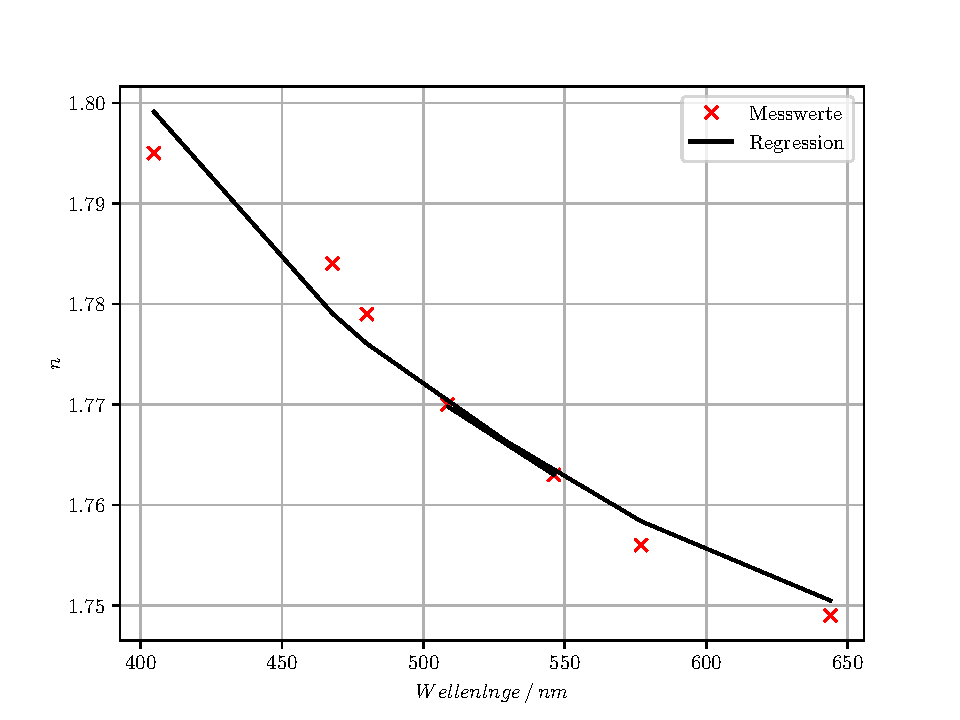
\includegraphics[width=\textwidth]{plot1.pdf}
  \caption{Darstellung der Dispersionskurven.}
  \label{abb:4}
\end{figure}
Die Ausgleichsrechnungen sind mit Python 3.6 durchgeführt worden. Dabei wurden
die Gleichungen \ref{eq:3} und \ref{eq:4} für die Regression verwendet.
Es ergeben sich für die Parameter folgende Werte:
\begin{itemize}
  \item $A_0 = \num{2.912(0072)}$
  \item $A_2 = \SI{58467.62(182582)}{\nano\meter}^2$
  \item $A'_0 = \num{3.334(027)}$
  \item $A'_2 = (7,121 \pm 0,9563)10^{-7} \si[per-mode=fraction]{\per\nano\meter\squared}$
\end{itemize}
Um nun bestimmen zu können, welche Fall für die Dispersionskurve genommen werden soll, wird
die Methode der kleinsten Quadrate verwendet.
\begin{equation}
  s^2_n = \frac{1}{z-2} \sum_{i=1}^{z}(n^2(\lambda_i)-A_0-\frac{A_2}{\lambda^2_i})^2 \,\,\, \text{für} \, \lambda >> \lambda_1
  \label{eq:10}
\end{equation}
\begin{equation}
  s^2_{n'} = \frac{1}{z-2} \sum_{i=1}^{z}(n^2(\lambda_i)-A'_0+A'_2 \cdot \lambda^2_i)^2 \,\,\, \text{für} \, \lambda << \lambda_1
  \label{eq:11}
\end{equation}
Die eingesetzten Werte in Gleichung \ref{eq:10} und \ref{eq:11} ergeben aufsummiert.
\begin{itemize}
  \item $s^2_n = \num{1.9286925(1)e-5}$
  \item $s^2_{n'} = \num{3.28783880(6)e-4}$
\end{itemize}
Da $s^2$ möglichst klein sein soll, wird die Formel \ref{eq:3} für $\lambda >> \lambda_1$ genutzt.
Es folgt für den Brechungsindex folgende Gleichung
\begin{equation}
  n(\lambda)= \sqrt{A_0 + \frac{A_2}{\lambda^2}}.
  \label{eq:12}
\end{equation}

Mithilfe der Dispersionsgleichung \ref{eq:12} wird die \textbf{Abbesche Zahl} bestimmt.
Sie sagt aus wie die Farbzerstreuung von dem \textbf{SF15} ist.
Die Gleichungen lautet
\begin{equation}
  \nu = \frac{n_D -1}{n_F-n_C}.
  \label{eq:13}
\end{equation}
Die Ergebnisse in der Tabelle \ref{tab:3}
dargestellt. Für die Wellenlänge werden die Fraunhoferschen Linien verwendet.
Der Fehler lässt sich mit der Gaußfehlerfortpflanzung
\begin{equation}
  \sigma^2 = \sum_i^N (\frac{\partial A_i}{\partial x_i})^2 \cdot (\Delta A_i)^2
  \label{fel:3}
\end{equation}
berechnen.
Es folgt somit für Gleichung \ref{eq:13}
\begin{equation*}
  \sigma_{n} = \sqrt{(\frac{\partial n}{\partial A_0} \cdot \sigma_{A_0})^2 + (\frac{\partial n}{\partial A_2} \cdot \sigma_{A_2})^2}
\end{equation*}
Mit
\begin{equation*}
  \frac{\partial n}{\partial A_0} = \frac{1}{2} \frac{1}{\sqrt{A_0 + \frac{A_2}{\lambda^2}}}
\end{equation*}
und
\begin{equation*}
  \frac{\partial n}{\partial A_2} = \frac{1}{2 \lambda^2} \frac{1}{\sqrt{A_0 + \frac{A_2}{\lambda^2}}}
\end{equation*}
\begin{table}[H]
  \centering
  \caption{Bestimmung der Brechungsindices mit den Fraunhoferschen Linien.}
  \label{tab:3}
  \begin{tabular}{c c c c }
    \toprule
    $\text{Linie}$ & $\text{Wellenlänge} \,/\,\si{\nano\meter}$ & $\text{Brechungsindex}$ &$n$\\
    \midrule
    $\lambda_C$ & 656 & $1,746 \pm 0,002$ & $n_C$\\
    $\lambda_D$ & 589 & $1,755 \pm 0,003$ & $n_D$\\
    $\lambda_F$ & 486 & $1,778 \pm 0,003$ & $n_F$\\
    \bottomrule
  \end{tabular}
\end{table}
Mit Gleichung \ref{eq:13} lautet die \textbf{Abbesche Zahl}
\begin{equation*}
  \nu = \num{23.8(7)}
\end{equation*}
Der Fehler ergibt sich mit \ref{fel:3} zu:
\begin{equation*}
  \sigma_\nu = \sqrt{(\frac{\partial \nu}{\partial n_D} \sigma_{n_D})^2 + (\frac{\partial \nu}{\partial n_f} \sigma_{n_f})^2 + (\frac{\partial \nu}{\partial n_c} \sigma_{n_c})^2}
\end{equation*}
Mit
\begin{equation*}
  \frac{\partial \nu}{\partial n_D} = \frac{1}{n_f - n_c}
\end{equation*}
\begin{equation*}
  \frac{\partial \nu}{\partial n_f} = -\frac{n_D - 1}{(n_f -n_c)^2}
\end{equation*}
\begin{equation*}
  \frac{\partial \nu}{\partial n_c} = \frac{n_D - 1}{(n_f -n_c)^2}
\end{equation*}
Für das Auflösungsvermögen werden zwei benachbarte Wellenlängen
als Wellenlängenunterschied $\Delta\lambda$ bezeichnet. Der Wellenlängeunterschied $\Delta\lambda$ muss
so gering sein, dass sie gerade vom Gerät getrennt werden können.
Der Ausdruck für das Auflösungsvermögen lautet
\begin{equation*}
  A = \frac{\lambda}{\Delta\lambda}
\end{equation*}
Durch Näherungen von Winkelfunktionen kann das Auflösungsvermögen umgeschrieben werden zu
\begin{equation}
  A = b \frac{d}{d\lambda} n(\lambda).
  \label{eq:14}
\end{equation}
Dabei ist $b$ die Basislänge vom Prisma und beträgt $\SI{3}{\centi\meter}$.
Nun wird die Gleichung \ref{eq:3} nach $\lambda$ abgeleitet und in die Gleichung \ref{eq:14}
eingesetzt.
Es folgt für das Auflösungsvermögen in Betrag:
\begin{equation}
  |A| = \frac{b \cdot A_2}{\lambda^3 \sqrt{A_0 +\frac{A_2}{\lambda^2}}}
\end{equation}
Die Ergebnisse werden in der Tabelle \ref{tab:4} dargestellt.
\begin{table}[H]
  \centering
  \caption{Auflösungsvermögen von den Fraunhoferschen Linien.}
  \label{tab:4}
  \begin{tabular}{c c c}
    \toprule
    $\text{Linie}$ & $\text{Wellenlänge} \,/\,\si{\nano\meter}$ & $\text{Auflösungsvermögen}$\\
    \midrule
    $\lambda_c$ & 656 & $\num{3558.86(10874)}$\\
    $\lambda_D$ & 589 & $\num{4890.60(14866)}$\\
    $\lambda_F$ & 486 & $\num{8596.08(25811)}$\\
    \bottomrule
  \end{tabular}
\end{table}
Mit der Gleichung \ref{fel:3} lautet der Fehler:
\begin{equation*}
  \sigma_A = \sqrt{(\frac{\partial A} {\partial A_0} \sigma_{A_0})^2 + (\frac{\partial A}{\partial A_2} \sigma_{A_2})^2}
\end{equation*}
Mit
\begin{equation*}
  \frac{\partial A} {\partial A_0} = -\frac{b\cdot A_2}{2\lambda^3 \sqrt{(A_0 + \frac{A_2}{\lambda^2})^3}}
\end{equation*}
\begin{equation*}
  \frac{\partial A}{\partial A_2} = \frac{b (A_2+2A_0\lambda^2)}{2\lambda^5 \sqrt{(A_0 + \frac{A_2}{\lambda^2})^3}}
\end{equation*}
Um nun die nächste abgelegene Absorptionstelle $\lambda_1$ zu bestimmen wird
mit der Lösung der Dispersionsgleichung ein Koeffizentenvergleich von $A_0 \, ,\, A_2$ mit
der Gleichung \ref{eq:3} durchgeführt.
Somit ergeben sich für
\begin{equation*}
  A_0 = 1 +\underbrace{\frac{N_h q_h^2}{4 \pi^2 c^2 \epsilon_0 m_h}}_\beta \lambda^2
  \label{eq:15}
\end{equation*}
und
\begin{equation*}
  A_2 = \beta \cdot \lambda_1^4.
  \label{eq:16}
\end{equation*}
Durch Auflösen von Gleichung \ref{eq:16} nach $\beta$ und Einsetzen in Gleichung \ref{eq:15} ergibt sich:
\begin{equation*}
  A_0 = 1+ \frac{A_2}{\lambda_1^2}
\end{equation*}
Durch Umformen nach der ersten Absorptionstelle $\lambda_1$ folgt:
\begin{equation*}
  \lambda_1 = \sqrt{\frac{A_2}{A_0-1}}
\end{equation*}
Die Werte eingesetzt ergibt sich zu:
\begin{equation*}
  \lambda_1 = \SI{174,9(27)}{\nano\meter}
\end{equation*}
Der Fehler wird mit Gleichung \ref{fel:3} berechnet.
Die Formel dazu lautet:
\begin{equation*}
  \sigma_{\lambda_1} = \sqrt{(\frac{d\lambda_1}{dA_0} \cdot \sigma_{A_0})^2 + (\frac{d\lambda_1}{dA_2} \cdot \sigma_{A_2})^2}
\end{equation*}
Mit
\begin{equation*}
  \frac{d\lambda_1}{dA_0} = -\frac{1}{2} (\frac{A_2}{A_0 -1})^{-\frac{1}{2}} \cdot \frac{A_2}{(A_0 - 1)^2}
\end{equation*}
und
\begin{equation*}
  \frac{d\lambda_1}{dA_2} = \frac{1}{2} (\frac{A_2}{A_0 -1})^{-\frac{1}{2}} \cdot \frac{1}{A_0 - 1}
\end{equation*}
